\documentclass[a4paper,10pt]{jsarticle}

% レイアウト
\setlength{\textwidth}{\fullwidth}
\setlength{\textheight}{39\baselineskip}
\addtolength{\textheight}{\topskip}
\setlength{\voffset}{-0.5in}
\setlength{\headsep}{0.3in}
\pagestyle{myheadings}

% パッケージ
\usepackage[dvipdfmx]{graphicx}
\usepackage{amsmath,amssymb,epsfig}
\usepackage{bm}
\usepackage{ascmac}
\usepackage{pifont}
\usepackage{multirow}
\usepackage{enumerate}
\usepackage{cases}
\usepackage{type1cm}
\usepackage{cancel}
\usepackage{url}
\usepackage{listings,jlisting}
% 大きな中括弧
\usepackage{cases}


% カウンタの設定
\setcounter{section}{0}
\setcounter{subsection}{0}
\setcounter{subsubsection}{0}
\setcounter{equation}{0}

% キャプションの図をFigに変更
\renewcommand{\figurename}{Fig.}
\renewcommand{\tablename}{Tab.}

% 式番号を式(章番号.番号)に
\makeatletter
\renewcommand{\theequation}{\arabic{section}.\arabic{equation}}
\@addtoreset{equation}{section}
\makeatother

% 表紙
\title{知能システム学特論レポート}
\author{
(DL2班)Caffe on Ubuntu\\
}
\date{2015年\ 6月\ 29日}

% ドキュメントの開始
\begin{document}
\maketitle
\section{報告者}
\begin{list}{}{}
 \item 15344203\hspace{0.5cm} 有田 裕太
 \item 15344206\hspace{0.5cm} 緒形 裕太
 \item 15344209\hspace{0.5cm} 株丹 亮
 \item 12104125\hspace{0.5cm} 宮本 和
\end{list}

\section{進行状況}

\begin{itemize}
\item 理論研究
\item 順伝播型ネットワークについて
\end{itemize}


\section{理論研究}
\subsection{ユニットの出力}

\subsection{活性化関数}

\subsection{多層ネットワーク}
Fig.~\ref{fig:2層のネットワーク}に2層構造のネットワークを示す.
Fig.~\ref{fig:2層のネットワーク}~(a)より各層を$l=0,\ 1,\ 2$とすると,$l=1$の層を入力層,$l=2$を中間層,隠れ層,$l=3$を出力層と呼ぶ.
各層のユニットの入出力を区別するために,入力を$\bm{u}^{(l)}$,出力を$\bm{z}^{(l)}$と定義すると,中間層($l=2$)のユニットの出力は以下の式で表される.
\begin{eqnarray}
\label{eq:3a}
  \bm{u}^{(2)} &=& \bm{W}^{(2)}\bm{x} + \bm{b}^{(2)} \\
  \bm{z}^{(2)} &=& \bm{f}(\bm{u}^{(2)})
\end{eqnarray}
$\bm{W}^{(2)}$は入力層と中間層の結合重みであり,$\bm{b}^{(2)}$は中間層のユニットに与えられたバイアスである.
同様にして$\bm{u}^{(3)}$,$\bm{z}^{(3)}$は
\begin{eqnarray}
\label{eq:3b}
  \bm{u}^{(3)} &=& \bm{W}^{(3)}\bm{z}^{(2)} + \bm{b}^{(3)} \\
  \bm{z}^{(3)} &=& \bm{f}(\bm{u}^{(3)})
\end{eqnarray}
となり,任意の階層$L$のネットワークに一般化すると
\begin{eqnarray}
\label{eq:3c}
  \bm{u}^{(l+1)} &=& \bm{W}^{(l+1)}\bm{z}^{(l)} + \bm{b}^{(l+1)} \\
  \bm{z}^{(l+1)} &=& \bm{f}(\bm{u}^{(l+1)})
\end{eqnarray}
と書ける.
$l=1,\ 2,\ 3,\cdots, L-1$の順に繰り返していくと最終的な出力$\bm{y}$を決定することができる.
この出力を決定するのは各層間の結合重み$\bm{W}^{(l)}\ (l=2,\cdots, L)$とユニットのバイアス$\bm{W}^{(l)}\ (l=2,\cdots, L)$である.
これらのパラメータを持つベクトル$\bm{w}$を定義して,$\bm{y}(\bm{x};\bm{w})$と表現する.

\begin{figure}[tb]
  \begin{center}
    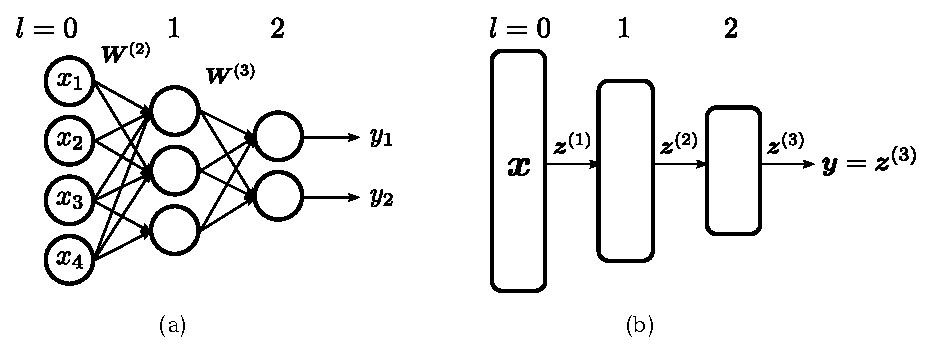
\includegraphics[clip,width=10cm]{fig/eps/unit.eps}
  \end{center}
  \caption{2層のネットワーク}
  \label{fig:2層のネットワーク}
\end{figure}

\subsection{出力層の設計と誤差関数}


\section{今後の課題}
\begin{itemize}
 \item 理論研究を進める.
 \item Caffeを使いこなす
\end{itemize}

\end{document}